\documentclass{beamer} 
\usepackage{tikz}
\usepackage[all]{xy}
\usepackage{amsmath,amssymb}
\usepackage{hyperref}
\usepackage{graphicx}
\usepackage{algorithmic}
\usepackage{multirow}

\DeclareMathOperator*{\argmin}{arg\,min}
\DeclareMathOperator*{\Lik}{Lik}
\DeclareMathOperator*{\PoissonLoss}{PoissonLoss}
\DeclareMathOperator*{\Peaks}{Peaks}
\DeclareMathOperator*{\Segments}{Segments}
\DeclareMathOperator*{\argmax}{arg\,max}
\DeclareMathOperator*{\maximize}{maximize}
\DeclareMathOperator*{\minimize}{minimize}
\newcommand{\sign}{\operatorname{sign}}
\newcommand{\RR}{\mathbb R}
\newcommand{\ZZ}{\mathbb Z}
\newcommand{\NN}{\mathbb N}
\newcommand{\z}{$z = 2, 4, 3, 5, 1$} 

\newcommand{\algo}[1]{\textcolor{#1}{#1}}
\definecolor{PDPA}{HTML}{66C2A5}
\definecolor{CDPA}{HTML}{FC8D62}
\definecolor{GPDPA}{HTML}{4D4D4D}

% Set transparency of non-highlighted sections in the table of
% contents slide.
\setbeamertemplate{section in toc shaded}[default][100]
\AtBeginSection[]
{
  \setbeamercolor{section in toc}{fg=red} 
  \setbeamercolor{section in toc shaded}{fg=black} 
  \begin{frame}
    \tableofcontents[currentsection]
  \end{frame}
}

\begin{document}

\title{Cross-validation for comparing qSIP prediction models trained
  on same or other groups}

\author{
  Toby Dylan Hocking\\
  toby.hocking@nau.edu\\
  toby.hocking@r-project.org\\
}

\maketitle


\begin{frame}
  \frametitle{Supervised learning for comparing }
\end{frame}

\begin{frame}
  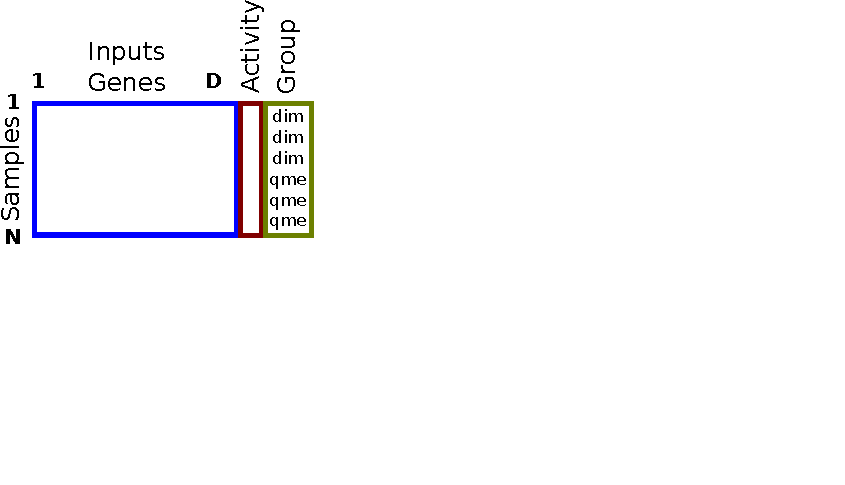
\includegraphics[width=\textwidth]{drawing-cv-same-other-1}
\end{frame}

\begin{frame}
  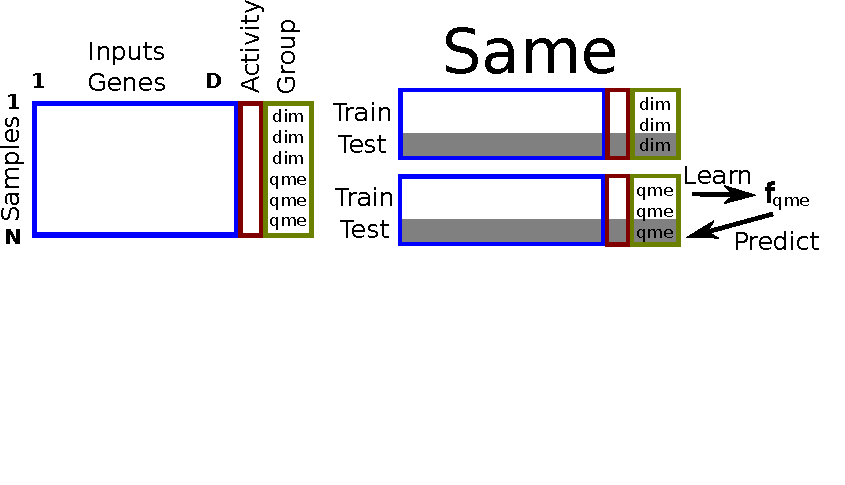
\includegraphics[width=\textwidth]{drawing-cv-same-other-2}
\end{frame}

\begin{frame}
  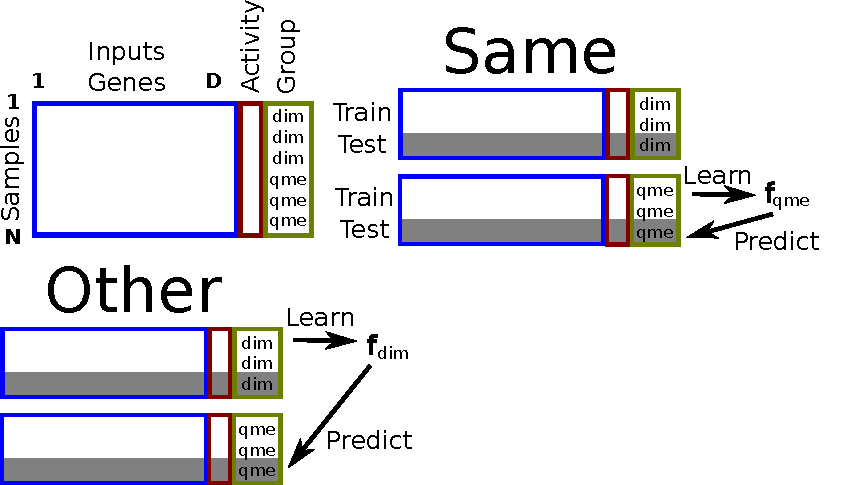
\includegraphics[width=\textwidth]{drawing-cv-same-other-3}
\end{frame}

\begin{frame}
  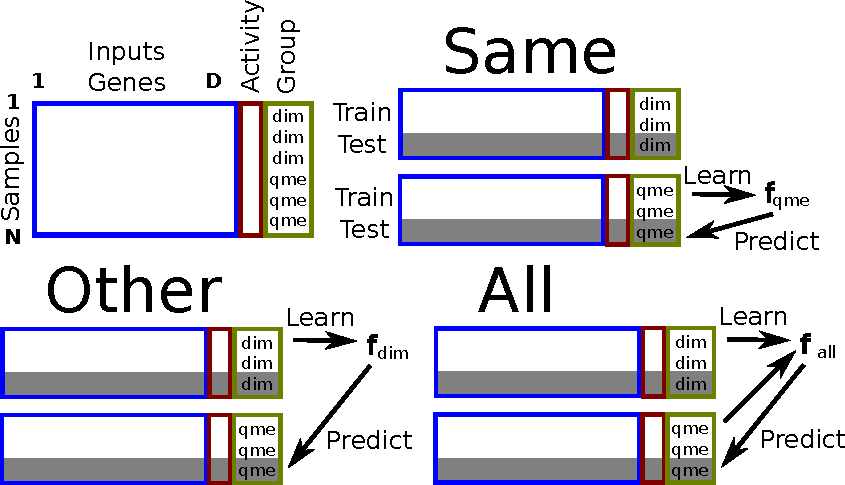
\includegraphics[width=\textwidth]{drawing-cv-same-other-4}
\end{frame}

\begin{frame}
  TODO same fig
\end{frame}

\begin{frame}
  TODO same+other fig
\end{frame}

\begin{frame}
  TODO same+other+all fig
\end{frame}

\begin{frame}
  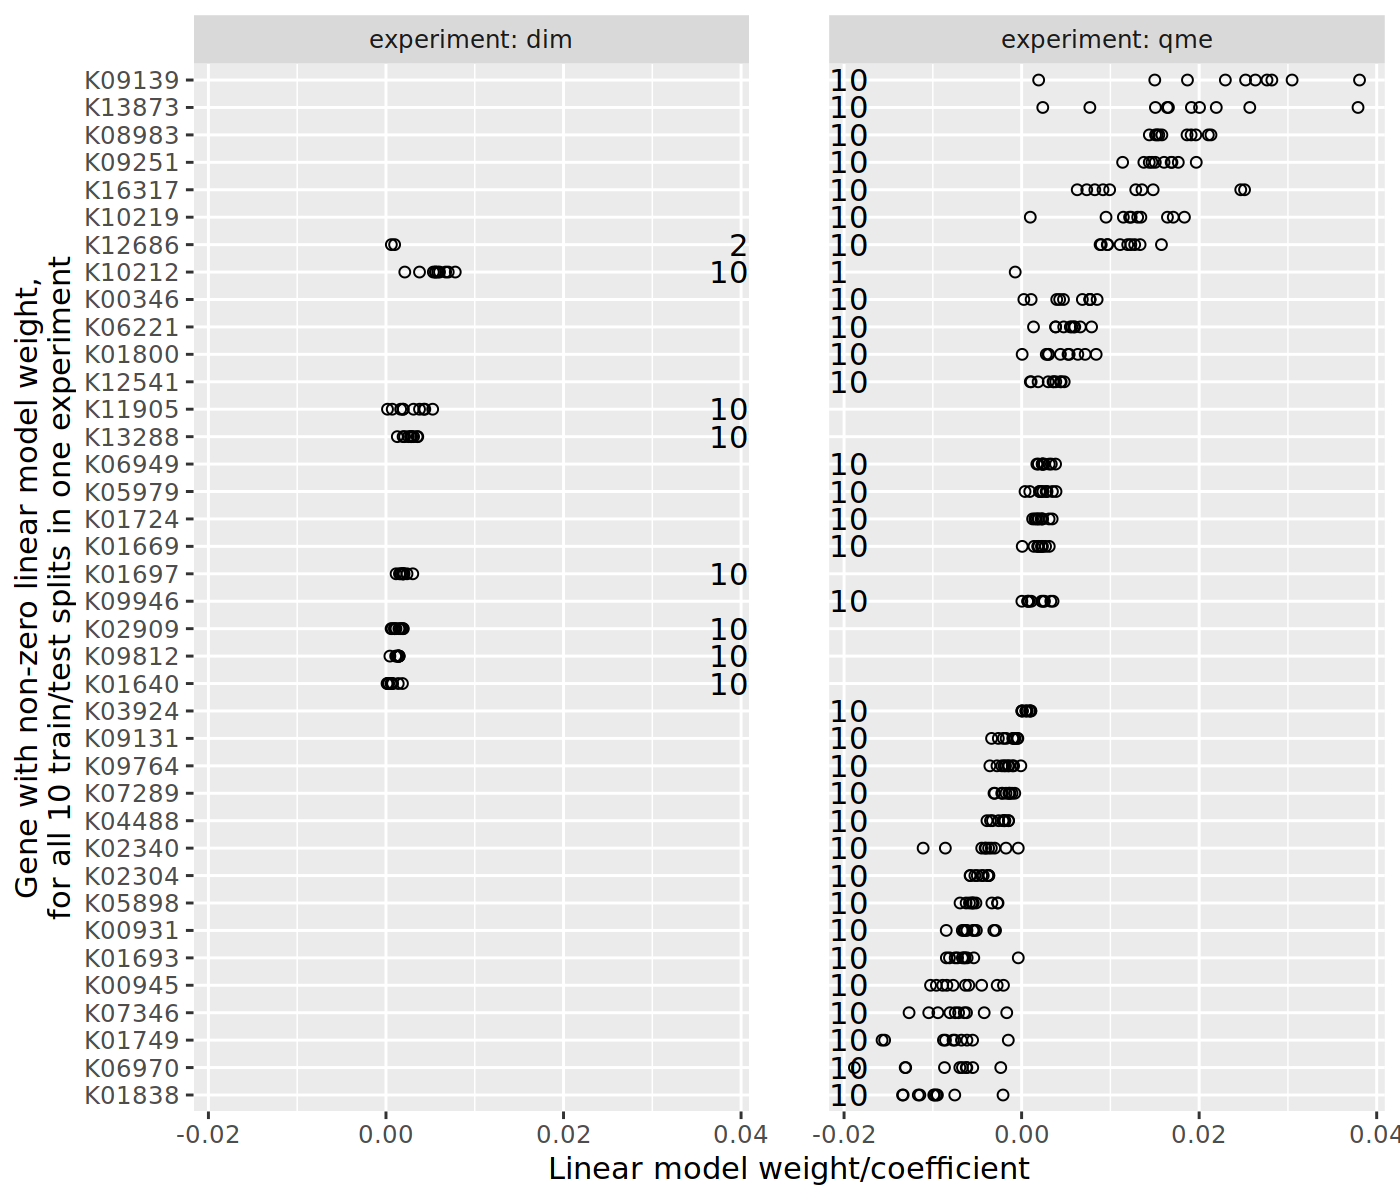
\includegraphics[width=\textwidth]{2024-01-09-qsip_pc2_all_new-controls.between.experiments.weights.png}
\end{frame}

\begin{frame}
  \frametitle{Discussion and conclusions}
  \begin{itemize}
  \item TODO
  \item Free/open-source software available: mlr3resampling R package.
  \end{itemize}
\end{frame}

\end{document}